\documentclass[12pt]{beamer}\usepackage[]{graphicx}\usepackage[]{color}
%% maxwidth is the original width if it is less than linewidth
%% otherwise use linewidth (to make sure the graphics do not exceed the margin)
\makeatletter
\def\maxwidth{ %
  \ifdim\Gin@nat@width>\linewidth
    \linewidth
  \else
    \Gin@nat@width
  \fi
}
\makeatother

\definecolor{fgcolor}{rgb}{0.345, 0.345, 0.345}
\newcommand{\hlnum}[1]{\textcolor[rgb]{0.686,0.059,0.569}{#1}}%
\newcommand{\hlstr}[1]{\textcolor[rgb]{0.192,0.494,0.8}{#1}}%
\newcommand{\hlcom}[1]{\textcolor[rgb]{0.678,0.584,0.686}{\textit{#1}}}%
\newcommand{\hlopt}[1]{\textcolor[rgb]{0,0,0}{#1}}%
\newcommand{\hlstd}[1]{\textcolor[rgb]{0.345,0.345,0.345}{#1}}%
\newcommand{\hlkwa}[1]{\textcolor[rgb]{0.161,0.373,0.58}{\textbf{#1}}}%
\newcommand{\hlkwb}[1]{\textcolor[rgb]{0.69,0.353,0.396}{#1}}%
\newcommand{\hlkwc}[1]{\textcolor[rgb]{0.333,0.667,0.333}{#1}}%
\newcommand{\hlkwd}[1]{\textcolor[rgb]{0.737,0.353,0.396}{\textbf{#1}}}%
\let\hlipl\hlkwb

\usepackage{framed}
\makeatletter
\newenvironment{kframe}{%
 \def\at@end@of@kframe{}%
 \ifinner\ifhmode%
  \def\at@end@of@kframe{\end{minipage}}%
  \begin{minipage}{\columnwidth}%
 \fi\fi%
 \def\FrameCommand##1{\hskip\@totalleftmargin \hskip-\fboxsep
 \colorbox{shadecolor}{##1}\hskip-\fboxsep
     % There is no \\@totalrightmargin, so:
     \hskip-\linewidth \hskip-\@totalleftmargin \hskip\columnwidth}%
 \MakeFramed {\advance\hsize-\width
   \@totalleftmargin\z@ \linewidth\hsize
   \@setminipage}}%
 {\par\unskip\endMakeFramed%
 \at@end@of@kframe}
\makeatother

\definecolor{shadecolor}{rgb}{.97, .97, .97}
\definecolor{messagecolor}{rgb}{0, 0, 0}
\definecolor{warningcolor}{rgb}{1, 0, 1}
\definecolor{errorcolor}{rgb}{1, 0, 0}
\newenvironment{knitrout}{}{} % an empty environment to be redefined in TeX

\usepackage{alltt}
\usepackage{tikz}

% make it pretty
% get rid of junk
\usetheme{default}
\usefonttheme[onlymath]{serif}
\beamertemplatenavigationsymbolsempty

% define a bunch of colors
\definecolor{offwhite}{RGB}{255,250,240}
\definecolor{gray}{RGB}{155,155,155}
\definecolor{foreground}{RGB}{80,80,80}
\definecolor{background}{RGB}{255,255,255}
%\definecolor{title}{RGB}{255,199,0}
\definecolor{title}{RGB}{89,132,212}
%\definecolor{subtitle}{RGB}{89,132,212}
\definecolor{subtitle}{RGB}{255,199,0}
\definecolor{hilit}{RGB}{248,117,79}
\definecolor{vhilit}{RGB}{255,111,207}
\definecolor{lolit}{RGB}{200,200,200}
\definecolor{lit}{RGB}{255,199,0}
\definecolor{mdlit}{RGB}{89,132,212}
\definecolor{link}{RGB}{248,117,79}

% a few color macros
\newcommand{\hilit}{\color{hilit}}
\newcommand{\vhilit}{\color{vhilit}}
\newcommand{\lit}{\color{lit}}
\newcommand{\mdlit}{\color{mdlit}}
\newcommand{\lolit}{\color{lolit}}

% use those colors
\setbeamercolor{titlelike}{fg=title}
\setbeamercolor{subtitle}{fg=subtitle}
\setbeamercolor{frametitle}{fg=gray}
%\setbeamercolor{structure}{fg=subtitle}
\setbeamercolor{structure}{fg=title}
\setbeamercolor{institute}{fg=lolit}
\setbeamercolor{normal text}{fg=foreground,bg=background}
\setbeamertemplate{itemize subitem}{{\textendash}}
\setbeamerfont{itemize/enumerate subbody}{size=\small}
\setbeamerfont{itemize/enumerate subitem}{size=\small}

% center title of slides
\setbeamertemplate{blocks}[rounded]
\setbeamertemplate{frametitle}[default][center]

% page number
\setbeamerfont{page number in foot}{size=\footnotesize}
\setbeamertemplate{footline}[frame number]

% default link color
\hypersetup{colorlinks, urlcolor={link}}

% a few macros
\newcommand{\code}[1]{\texttt{#1}}
\newcommand{\hicode}[1]{{\hilit \texttt{#1}}}
\newcommand{\locode}[1]{{\lolit \texttt{#1}}}
\newcommand{\bb}[1]{\begin{block}{#1}}
\newcommand{\eb}{\end{block}}
\newcommand{\bi}{\begin{itemize}}
\newcommand{\bbi}{\vspace{4pt} \begin{itemize} \itemsep8pt}
\newcommand{\ei}{\end{itemize}}
\newcommand{\bv}{\begin{verbatim}}
\newcommand{\ev}{\end{verbatim}}
\newcommand{\ig}{\includegraphics}
\newcommand{\subt}[1]{{\footnotesize \color{subtitle} {#1}}}
\newcommand{\ttsm}{\tt \small}
\newcommand{\ttfn}{\tt \footnotesize}
\newcommand{\figh}[2]{\centerline{\includegraphics[height=#2\textheight]{#1}}}
\newcommand{\figw}[2]{\centerline{\includegraphics[width=#2\textwidth]{#1}}}



%------------------------------------------------

\title{Graphing Process}
\subtitle{Intro to Data Visualization}
\author{\href{http://www.gastonsanchez.com}{Gaston Sanchez}}
\institute{\href{https://creativecommons.org/licenses/by-sa/4.0/}{\tt \scriptsize \color{foreground} CC BY-SA 4.0}}
\date{}
\IfFileExists{upquote.sty}{\usepackage{upquote}}{}
\begin{document}

% no page number in first slide
{
  \setbeamertemplate{footline}{} 
  \frame{\titlepage} 
}

%------------------------------------------------

\begin{frame}
\begin{center}
\Huge{\hilit{Cycle of Data Analysis Projects}}
\end{center}
\end{frame}

%------------------------------------------------

\begin{frame}
\frametitle{Cycle of Data Anlaysis Projects}
\begin{center}
\ig[width=7cm]{images/data-analysis-cycle.png}
\end{center}
\end{frame}

%------------------------------------------------

\begin{frame}
\frametitle{Cycle of DAP and data visualizations}

\bbi
  \item Data visualization may be present at any stage of a data analysis 
project (DAP).
  \item The data preparation stage is usually supported with quick check-up displays.
  \item Exploratory displays constantly appear in the actual data analysis part.
  \item Communication displays are central to the reporting stage.
\ei

\end{frame}

%------------------------------------------------

\begin{frame}
\begin{center}
\Huge{\hilit{Understanding the Data Analysis Process}}
\end{center}
\end{frame}

%------------------------------------------------

\begin{frame}[fragile]
\begin{center}
\ig[width=11cm]{images/data-by-the-numbers.png}

{\tiny \url{http://www.phdcomics.com/comics/archive.php/archive/tellafriend.php?comicid=462}}
\end{center}
\end{frame}

%------------------------------------------------

\begin{frame}[fragile]
\frametitle{Data Preparation}
\begin{center}
\ig[width=4cm]{images/databynumbers1.pdf}
\end{center}
\end{frame}

%------------------------------------------------

\begin{frame}[fragile]
\frametitle{Core Data Analysis}
\begin{center}
\ig[width=4cm]{images/databynumbers2.pdf}
\end{center}
\end{frame}

%------------------------------------------------

\begin{frame}[fragile]
\frametitle{Reporting}
\begin{center}
\ig[width=4cm]{images/databynumbers3.pdf}
\end{center}
\end{frame}

%------------------------------------------------

\begin{frame}[fragile]
\frametitle{Communication}
\begin{center}
\ig[width=4cm]{images/databynumbers4.pdf}
\end{center}
\end{frame}

%------------------------------------------------

\begin{frame}[fragile]
\begin{center}
\ig[width=8cm]{images/theory-practice.pdf}
\end{center}
\end{frame}

%------------------------------------------------

\begin{frame}
\begin{center}
\Huge{\hilit{Data Visualization Process}}
\end{center}
\end{frame}

%------------------------------------------------

\begin{frame}
\frametitle{Datavis Process}

\bb{Main Considerations}
The plotting steps vary by dataset and project. But you should consider:
\begin{enumerate}
  \item What data do you have?
  \item What do you want to know about the data?
  \item What visualization methods should you use?
  \item What do you see and does it make sense?
\end{enumerate}
\eb

\end{frame}

%------------------------------------------------

\begin{frame}[fragile]
\frametitle{Exploration Process}
\begin{center}
\ig[width=10cm]{images/exploration-process.pdf}

{\scriptsize {\lolit (based on Nathan Yau)}}
\end{center}
\end{frame}

%------------------------------------------------

\begin{frame}[fragile]
\frametitle{Exploration Process}
\begin{center}
\ig[width=10cm]{images/exploration-process1.pdf}
\end{center}
\end{frame}

%------------------------------------------------

\begin{frame}
\frametitle{What data you have?}

\bbi
  \item Garbage in $\Rightarrow$ Garbage out.
  \item Good visualizations depend on good data.
  \item Data: can be small, medium, large, big.
  \item The important thing is its quality.
\ei

\end{frame}

%------------------------------------------------

\begin{frame}[fragile]
\frametitle{Exploration Process}
\begin{center}
\ig[width=10cm]{images/exploration-process2.pdf}
\end{center}
\end{frame}

%------------------------------------------------

\begin{frame}
\frametitle{What do you want to know?}

\bbi
  \item What is the research question?
  \item Focus on one or two questions that you want to answer.
  \item Talk with the experts in the field of application.
  \item At the beginning of a project, there will be more exploratory tasks.
  \item As a project evolves, the more refined and targeted the visualizations.
\ei

\end{frame}

%------------------------------------------------

\begin{frame}[fragile]
\frametitle{Exploration Process}
\begin{center}
\ig[width=10cm]{images/exploration-process3.pdf}
\end{center}
\end{frame}

%------------------------------------------------

\begin{frame}
\frametitle{What visualization to use?}

\bi
  \item How many variables?
  \bi
    \item One variable
    \item Two variables
    \item Three or more
  \ei
  \item What type of variables?
  \item Quantitative, qualitative, time
\ei

\end{frame}

%------------------------------------------------

\begin{frame}
\frametitle{What visualization to use?}

\bi
  \item Distributions
  \item Parts of a whole
  \item Trends in time
  \item Maps and geographic displays
  \item Bivariate Relationships
  \item Networks and other associations
  \item Facetting
\ei

\end{frame}

%------------------------------------------------

\begin{frame}[fragile]
\frametitle{Exploration Process}
\begin{center}
\ig[width=10cm]{images/exploration-process4.pdf}
\end{center}
\end{frame}

%------------------------------------------------

\begin{frame}
\frametitle{What do you see?}

\bb{Things to pay attention to:}
\bi
  \item Systematic variation
  \item Increasing patterns
  \item Decreasing patterns
  \item Atypical values (outliers)
  \item Similarities and differences
\ei
\eb

\end{frame}

%------------------------------------------------

\begin{frame}[fragile]
\frametitle{Exploration Process}
\begin{center}
\ig[width=10cm]{images/exploration-process.pdf}
\end{center}
\end{frame}

%------------------------------------------------

\begin{frame}
\frametitle{Visualization Process}

\bi
  \item Iterative Process
  \item Back and Forth
  \item Trial and Error
  \item Target questions
\ei

\end{frame}

%------------------------------------------------

\begin{frame}
\begin{center}
\Huge{\hilit{Things to keep in mind}}
\end{center}
\end{frame}

%------------------------------------------------

\begin{frame}
\frametitle{It's (almost) all about the questions}

\bbi
  \item Great visualization never start from the standpoint of the data set.
  \item Great visualization starts with questions.
  \item Why was the data collected?
  \item What is interesting about the data set?
  \item What stories can it tell?
\ei

\end{frame}

%------------------------------------------------

\begin{frame}
\frametitle{It's (almost) all about the questions}

\bbi
  \item An fundamental skill in understanding data is asking good questions.
  \item Identify the question that you want to answer.
  \item Think about how it will be used and work backward to what was collected.
  \item The more specific the question, the better visualizations tend to be.
\ei

\end{frame}

%------------------------------------------------

\begin{frame}
\begin{center}
\Huge{\hilit{Data Visualization Purposes}}
\end{center}
\end{frame}

%------------------------------------------------

\begin{frame}
\frametitle{Stats Graphics}

\centerline{\mdlit \Large Graphics for}

\bigskip
\centerline{\Large Exploration \quad \& \quad Communication}

\end{frame}

%------------------------------------------------

\begin{frame}
\frametitle{Analysis and Exploration}

\bb{Graphics for Exploration}
\bbi
  \item Graphics for understanding data.
  \item The analyst is the main (and usually only) consumer.
  \item Typically quick \& dirty.
  \item Not much care about visual appearance and design principles.
  \item Lifespan of a few seconds.
  \item Basic plots (deault parameters) in R are designed for this purpose.
\ei
\eb

\end{frame}

%------------------------------------------------

\begin{frame}
\frametitle{Graphics for Exploration Example}

\begin{knitrout}
\definecolor{shadecolor}{rgb}{0.969, 0.969, 0.969}\color{fgcolor}

{\centering 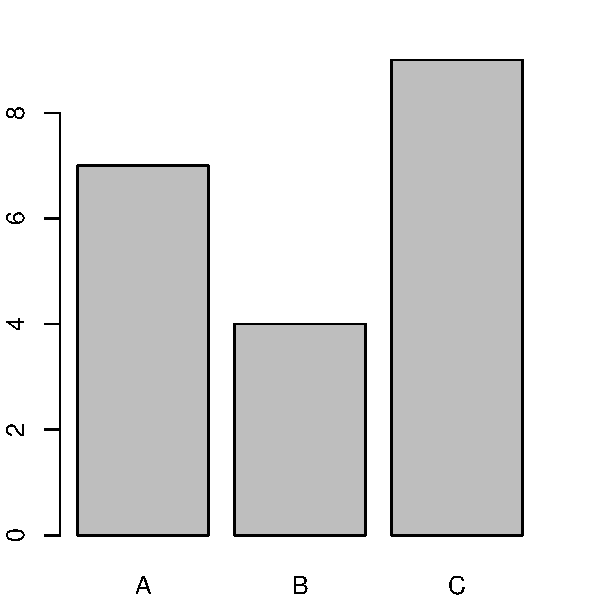
\includegraphics[width=.7\linewidth,height=.6\linewidth]{figure/unnamed-chunk-1-1} 

}



\end{knitrout}

\end{frame}

%------------------------------------------------

\begin{frame}
\frametitle{Communication and Presentation}

\bb{Graphics for Communication}
\bi
  \item Graphics for presenting data
  \item To be consumed by others
  \item Must care about visual appearance and design
  \item Require a lot of iterations in order to get the final version
  \item What's the message? 
  \item Who's the audience?
  \item On what type of media / format?
  \item Very time consuming!
\ei
\eb

\end{frame}

%------------------------------------------------

\begin{frame}
\frametitle{Graphics for Communication}

\begin{knitrout}
\definecolor{shadecolor}{rgb}{0.969, 0.969, 0.969}\color{fgcolor}

{\centering 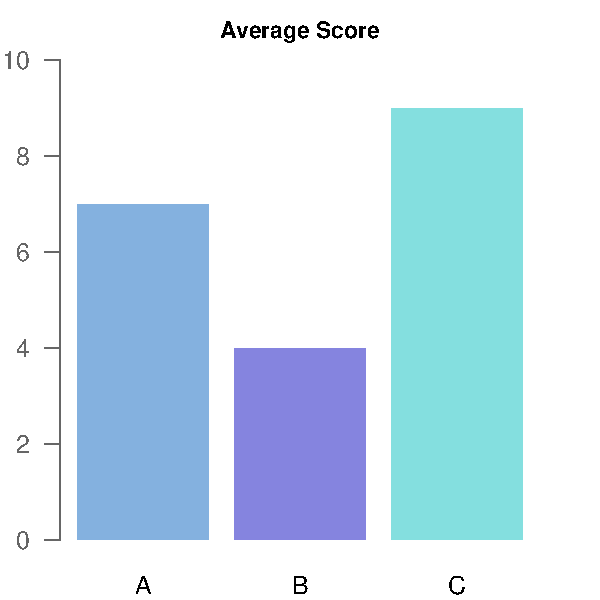
\includegraphics[width=.7\linewidth,height=.6\linewidth]{figure/unnamed-chunk-2-1} 

}



\end{knitrout}

\end{frame}

%------------------------------------------------

\begin{frame}
\frametitle{Graphics for Communication}

Use visualization to communicate ideas, influence, explain persuade

\bigskip
Visuals can serve as evidence or support

\end{frame}

%------------------------------------------------

\begin{frame}
\begin{center}
\Huge{\hilit{Graphical output in different formats}}
\end{center}
\end{frame}

%------------------------------------------------

\begin{frame}
\frametitle{Plotting options}

\centerline{\Large \mdlit When creating a plot in R ...}

\vspace{18pt}

\centerline{\Large Screen display \quad OR \quad Save in File}

\end{frame}

%------------------------------------------------

\begin{frame}
\frametitle{File Acronyms}

\begin{center}
  \begin{tabular}{l l}
  \multicolumn{2}{c}{\textbf{File Acronyms}} \\
  \hline
  Acronym & Description \\
    \hline
    PDF & Portable Document Format \\
    SVG & Scalable Vector Graphics \\
    PNG & Portable Network Graphics \\
    JPEG & Joint Photographic Experts Group \\
    BMP & Bitmap \\
    TIFF & Tagged Image File Format \\
    \hline
 \end{tabular}
\end{center}

\end{frame}

%------------------------------------------------

\begin{frame}
\frametitle{Output Formats}

\centerline{\Large \mdlit Graphics devices from the output format}

\bigskip

\centerline{\Large Vector \quad -vs- \quad Raster}

\end{frame}

%------------------------------------------------

\begin{frame}
\frametitle{Output Formats}

\bb{Vector Formats}
An image is described by a set of mathematical shapes (e.g. PDF, PostScript, SVG)
\eb

\bb{Raster Formats}
An image consists of an array of pixels, with information such as color recorded for each pixel (e.g. PNG, JPEG, TIFF, all screen devices)
\eb

\end{frame}

%------------------------------------------------

\begin{frame}
\frametitle{Vector or Raster?}

\bb{Vector Formats}
Vector formats are superior for images that need to be viewed at a variety of scales (i.e. zoom in and out).
\eb

\end{frame}

%------------------------------------------------

\begin{frame}
\frametitle{Example: vector image (pdf)}
\begin{center}
\ig[width=7cm]{images/dummy_plot.pdf}
\end{center}
\end{frame}

%------------------------------------------------

\begin{frame}
\frametitle{Vector or Raster?}

\bb{Raster Formats}
Raster formats tend to be preferred when a plot is visually complex (e.g. many data points), and it will produce smaller files if the image is very complex.
\eb

\end{frame}

%------------------------------------------------

\begin{frame}
\frametitle{Example: raster image (png)}
\begin{center}
\ig[width=7cm]{images/dummy_plot.png}
\end{center}
\end{frame}

%------------------------------------------------

\begin{frame}
\frametitle{Vector or Raster?}

If further modifications to an R plot will be made using third-party software:
\bi
  \item removing a particular form are only possibe with vector format
  \item modifying pixels of a particular color are only possible with raster formats
\ei

{\lit Keep in mind: It is easy to convert a vector format to a raster format, while the reverse is almost impossible}

\end{frame}

%------------------------------------------------

\begin{frame}
\frametitle{Vector Formats}

\bb{PDF}
\bi
  \item Good choice of static format
  \item Resizes well, usually portable
  \item Less efficient if a plot has many objects/points
\ei
\eb

\end{frame}

%------------------------------------------------

\begin{frame}
\frametitle{Vector Formats}

\bb{SVG}
\bi
  \item XML-based format
  \item Good choice for web pages
  \item \code{svg()} available in Linux and Mac
  \item SVG output in Windows requires package \code{"Cairo"}
  \item Some advanced SVG features are limitted in R
\ei
\eb

\end{frame}

%------------------------------------------------

\begin{frame}
\frametitle{Raster (Bitmap) Formats}

\bb{PNG}
\bi
  \item Desirable format for simple images (most statistical graphics)
  \item Good for line drawings or images with solid colors
  \item Good for many, many objects, points=
  \item PNG uses \textbf{lossless} compression: compresses the image without losing information
  \item PNG does not resize well
  \item Consequently, PNG files can be edited without reducing quality
  \item Most web browsers can read this format natively
\ei
\eb

\end{frame}

%------------------------------------------------

\begin{frame}
\frametitle{Raster Formats}

\bb{JPEG}
\bi
  \item Good for photographs or natural scenes
  \item JPEG uses \textbf{lossy} compression: compresses the image with some information loss
  \item Consequently, repeatedly editing a JPEG filewill result in quality reduction
  \item JPEG does not resize well
  \item Better suited for complex images with lots of different regions (like photographs)
\ei
\eb

\end{frame}

%------------------------------------------------

\begin{frame}
\frametitle{Raster Formats}

\bb{TIFF}
\bi
  \item Sophisticated format that allows multiple pages of raster 
  output within a single file
  \item Supports lossless compression
  \item Less supported by web browsers
  \item Preferred format for publishers of books or journal articles
\ei
\eb

\end{frame}

%------------------------------------------------

\begin{frame}
\frametitle{Raster Formats}

\bb{Image Size}
\bi
  \item Size of Raster images is specified in number of pixels 
  (rahter than physical size in inches)
  \item The physical size of a raster image is determined by the 
  \textbf{resolution} at which it is viewed
  \item e.g. PNG image 72 pixels wide will be 1 inch wide when viewed 
  on a screen with a resolution of 72 dpi (dots per inch)
  \item e.g. PNG image 72 pixels wide will be 0.75 inches wide on a screen 
  with a resolution of 96 dpi
\ei
\eb

\end{frame}

%------------------------------------------------

\begin{frame}[c]
\frametitle{Considerations}

\centering
{\Large \mdlit Plots on Screen}

\vspace{18pt}

-vs-

\vspace{18pt}

{\Large \mdlit Plots on Print}

\end{frame}

%------------------------------------------------

\begin{frame}
\frametitle{David Smith's Recommendations}

\bi
  \item Use pdf for printing
  \item Use png for web displays
  \item For documents or for detail, go hi-resolution
  \item Choose your dimensions carefully
  \item Think about aspect ratio
  \item Vector formats are good for line drawings and plots with solid colors
  \item Remove the outer margins, if you're not using them
  \item Make sure anti-aliasing is enabled
  \item Avoid using JPEG
  \item Be creative
\ei

{\tiny \url{http://blog.revolutionanalytics.com/2009/01/10-tips-for-making-your-r-graphics-look-their-best.html}}

\end{frame}

%------------------------------------------------

\begin{frame}
\frametitle{PDF}

\bb{Use pdf for printing}
\bi
  \item Use pdf if you plan to print your graphic
  \item The graphic is scale-independent
  \item PDF viewers are ubiquitous these days
  \item Easy to create a high-quality printout of a PDF file on almost any printer
  \item Best choice whenever you want to send the graph as a file via email, 
  and the recipient needs the best quality possible
\ei
\eb

\end{frame}

%------------------------------------------------

\begin{frame}
\frametitle{PNG}

\bb{For Web display, use PNG}
\bi
  \item These days, the best choice is the PNG format
  \item Most browsers can display PNG graphics without trouble
  \item The main choice you need to make when using \code{png()} is the 
  dimensions of the graphic in pixels
  \item Slides 4x3 png plots: \code{width=1024} and \code{height=768} pixels
  \item Slides 16x9 png plots: \code{width=1920} and \code{height=1080} pixels
\ei
\eb

\end{frame}

%------------------------------------------------

\begin{frame}
\frametitle{Dimensions}

\bb{Choosing dimensions}
\bi
  \item For PDF graphs this is easiest to deal with, where you specify width 
  and height in inches anyway
  \item For raster images is a bit trickier:
  \item R assumes 72 pixels to the inch
  \item When you increase the pixel dimensions you're also increasing the 
  implicit size of the graph area
\ei
\eb

\end{frame}

%------------------------------------------------

\begin{frame}
\frametitle{Summary}

\bi
  \item Plots are created on a graphics device
  \item There are screen devices and file devices
  \item Default graphics on screen are good for exploratory analysis
  \item File devices are useful for presentation-consumption of graphics
  \item File devices are divided in \textit{Vector} and \textit{Raster} formats
  \item Vector formats are good for line drawings and plots with solid colors
  \item Bitmap formats are good for plots with a large number of points
\ei

\end{frame}

%------------------------------------------------

\end{document}
